\begin{flushright} {\tiny {\color{gray} (tikz\_P2.tex)}} \end{flushright}
%~~~~~~~~~~~~~~~~~~~~~~~~~~~~~~~~~~~~~~~~~~~~~~~~~~~~~~~~~~~~~~~~~~~~~~~~~~~~~~~~~~~~~~~~~~~~~~~~~~

\begin{center}
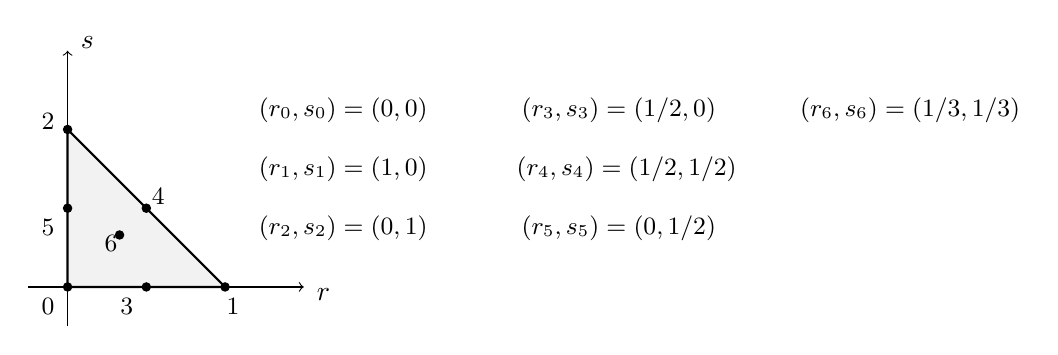
\begin{tikzpicture}
%\draw[step=0.5cm,gray,very thin] (0,0) grid (4,4); 
\draw[fill=gray!10,gray!10] (0.5,0.5)--(2.5,0.5)--(0.5,2.5)--cycle;
\draw[thick] (0.5,0.5)--(2.5,0.5)--(0.5,2.5)--cycle;
\draw [->] (0,0.5) -- (3.5,0.5);
\draw [->] (0.5,0) -- (0.5,3.5);
\node[] at (3.75,0.4) {$r$};
\node[] at (0.75,3.6) {$s$};
\draw[black,fill=black] (0.5,0.5)   circle (1.5pt);
\draw[black,fill=black] (2.5,0.5)   circle (1.5pt);
\draw[black,fill=black] (0.5,2.5)   circle (1.5pt);
\draw[black,fill=black] (1.5,0.5)   circle (1.5pt);
\draw[black,fill=black] (0.5,1.5)   circle (1.5pt);
\draw[black,fill=black] (1.5,1.5)   circle (1.5pt);
\draw[black,fill=black] (1.16,1.16) circle (1.5pt);

\node[] at (0.25,0.25) {\small $0$};
\node[] at (2.6,0.25)  {\small $1$};
\node[] at (0.25,2.6)  {\small $2$};
\node[] at (1.25,0.25) {\small $3$};
\node[] at (1.65,1.65) {\small $4$};
\node[] at (0.25,1.25) {\small $5$};
\node[] at (1.05,1.05)   {\small $6$};

\node[] at (4,2.75) {\small $(r_0,s_0)=(0,0)$};
\node[] at (4,2)    {\small $(r_1,s_1)=(1,0)$};
\node[] at (4,1.25) {\small $(r_2,s_2)=(0,1)$};
\node[] at (7.5,2.75) {\small $(r_3,s_3)=(1/2,0)$};
\node[] at (7.6,2)    {\small $(r_4,s_4)=(1/2,1/2)$};
\node[] at (7.5,1.25) {\small $(r_5,s_5)=(0,1/2)$};
\node[] at (11.2,2.75) {\small $(r_6,s_6)=(1/3,1/3)$};
\end{tikzpicture}
\end{center}

